\begin{table}
\centering
\begin{tabular}{l rrrrrr c}
\toprule
{\bf Št. glagolov} & {\bf 0} & {\bf 1} & {\bf 2} & {\bf 3} & {\bf 4} & {\bf $\geq$ 5} & {\bf $\sum$} \\
\midrule
{\bf Korpus}        & 1113,0 & 2680,0 & 1010,0 & 164,0 &  18,0 &  6,0 & 5000 \\
{\bf UMDHMM}        & 2094,2 & 1691,2 &  806,8 & 288,8 &  81,4 & 37,6 & 5000 \\
{\bf Lastna impl.}  & 1865,2 & 1733,6 &  897,8 & 344,6 & 110,8 & 48,0 & 5000 \\
{\bf hmmlearn}      & 1898,8 & 1717,6 &  880,4 & 346,2 & 107,4 & 49,6 & 5000 \\
\bottomrule
\end{tabular}
\caption{Porazdelitev glagolov pri izvornem besedilu in pričakovana
  porazdelitev glagolov za posamezna orodja.}
\label{tab:bench_model_table}
\end{table}

\begin{figure}
\begin{center}
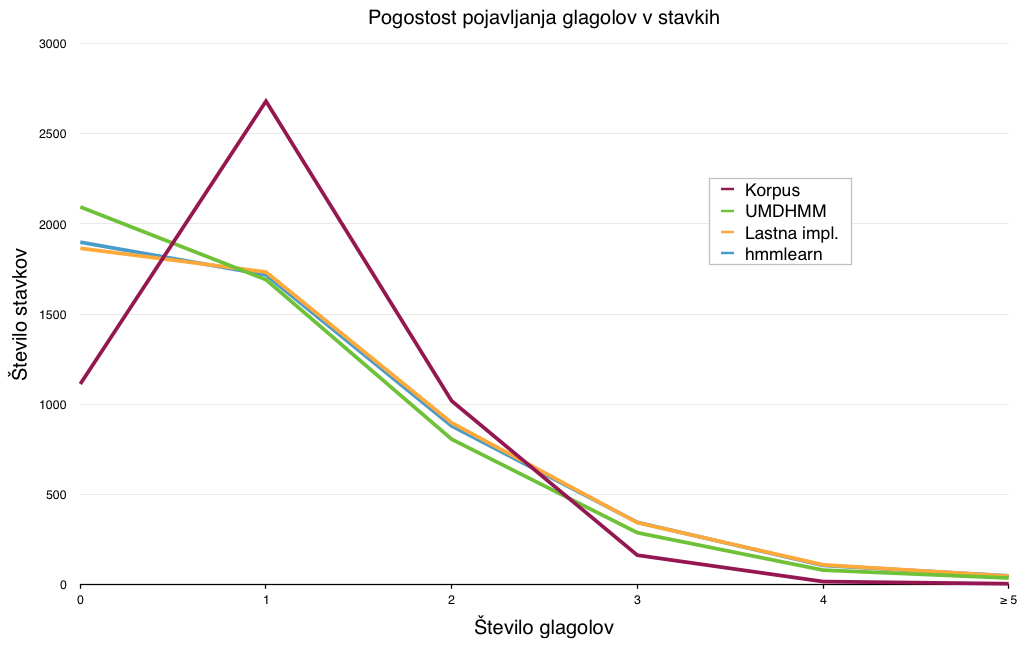
\includegraphics[width=\textwidth]{images/bench_model_comparison.png}
\end{center}
\caption{Pogostost pojavljanja glagolov pri različnih modelih.}
\label{fig:bench_model_comparison}
\end{figure}
